\clearpage
\section{Нейронные сети}
	В общем смысле, искусственная нейронная сеть - это математическая модель, построенная по принципу организации и функционирования биологических нейронных сетей. Она представляет из себя систему соединенных простых блоков - искусственных нейронов, каждый из которых имеет входы и выходы для взаимодействия с другими нейронами. Главное преимущество нейронных сетей перед традиционными алгоритмами в том, что они обучаются на некотором наборе данных, а не программируются в классическом смысле этого понятия. Процесс обучения заключается в нахождении оптимальных весовых коэффициентов между нейронами. С математической точки зрения, процесс обучения - это задача многопараметрической нелинейной оптимизации.
	\subsection{Математическая модель нейрона}
		Одиночный нейрон обычно представляет собой взвешенный сумматор с нелинейной функцией активации на выходе:
		$$x_{out} = \phi(\vec{w} \cdotp \vec{x}_{in}),$$
		где $\vec{w}$ - вектор весовых коэффициентов связей, $\vec{x}_{in}$ - входной вектор, $\phi$ - нелинейная функция активации (Рис. \ref{3-artificial-neuron-model}).
		
		\begin{figure}[h]
			\centering{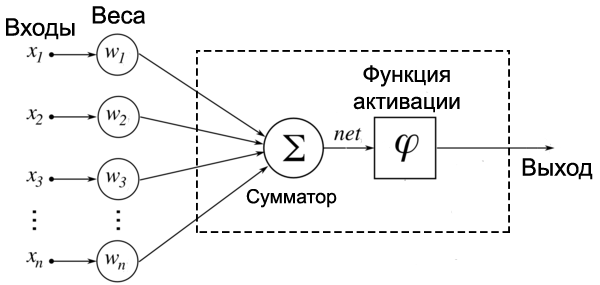
\includegraphics[width=0.9\linewidth]{3-ann/artificial-neuron-model}}
			\caption{Математическая модель нейрона}
			\label{3-artificial-neuron-model}
		\end{figure}
		
		Функция активации может выбираться разной в зависимости от задачи. Наиболее часто используемые функции:
		
		\begin{itemize}
			\item Сигмоида (логистическая функция)
					$$\sigma(x) = \frac{1}{1 + e^{-x}}$$
			\item Гиперболический тангенс
			\item ReLU
					$$ReLU(x) = \max(0, x)$$
			\item softmax
					$$\sigma(\vec{x})_j = \frac{e^{x_j}}{\sum_{k=1}^{N} e^{z_k}}$$
		\end{itemize}
		Множество таких нейронов объединяется в сеть и обучается каким-либо методом оптимизации.
	\subsection{Метод обратного распространения ошибки}
		Метод обратного распространения ошибки (backpropagation) - самый широко используемый и успешный алгоритм обучения глубоких (многослойных) нейронных сетей. Суть этого метода заключается в распространении сигналов ошибки от выходов сети к ее входам в обратном к распространению сигнала в сети направлении. Это позволяет вычислить производные ошибки по весам сети, которые потом можно использовать в любом градиентном алгоритме оптимизации (например, в стохастическом градиентном спуске).
		
		Обозначим множество входов сети как $\{x_1, \ldots, x_n\}$, множество выходов - $O$, $w_{ij}$ - вес, присвоенный ребру, соединяющему $i$-й и $j$-й узлы, $y_k$ - известные (правильные) ответы, $o_i$ - выход $i$-го узла. Введем функцию ошибки (например, сумма квадратов расстояний):
		$$ L(\vec{x}, W) = \frac{1}{2} \sum_{k \in O} (y_k - o_k)^2, $$
		где $W = \{w_{ij}\}$ - матрица весовых коэффициентов
		
		Рассмотрим сначала нейроны последнего слоя. Весовой коэффициент $w_{ij}$ влияет на выход сети как часть суммы $S_j = \sum_i w_{ij} x_i$. Соответственно,
		$$ \frac{\partial L}{\partial w_{ij}} = \frac{\partial L}{\partial S_j} \frac{\partial S_j}{\partial w_{ij}} = x_i \frac{\partial L}{\partial S_j} $$
		
		Аналогично, $S_j$ влияет на общую ошибку только в рамках выхода $j$-го узла $o_j$, поэтому
		$$ \frac{\partial L}{\partial S_j} = \frac{\partial L}{\partial o_j} \frac{\partial o_j}{\partial S_j}  = \left(\frac{\partial}{\partial o_j} \frac{1}{2} \sum_{k \in Out} (y_k - o_k)^2 \right) \left(\frac{\partial \phi(S)}{\partial S} \bigg|_{S = S_j} \right)$$
		Если узел $j$ не находится на последнем слое, то у него есть набор связей с нейронами следующего слоя. Обозначим их множество как $K_j$. Тогда
		$$ \frac{\partial L}{\partial S_j} = \sum_{k \in K_j} \frac{\partial L}{\partial S_k} \frac{\partial S_k}{\partial S_j} $$
		$$ \frac{\partial S_k}{\partial S_j} = \frac{\partial S_k}{\partial o_j} \frac{\partial o_j}{\partial S_j} = w_{jk}\frac{\partial o_j}{\partial S_j} $$
		$ \frac{\partial L}{\partial S_k}$ - аналогичная поправка, но для нейрона следующего слоя. В итоге, получены выражения для производных ошибки по весам для нейронов выходного слоя, а аналогичные производные для нейронов внутренних слоев выражены через нейроны следующих слоев. Это и есть процесс обратного распространения ошибки - градиенты ошибки по весам вычисляются последовательно, начиная с выходного слоя и заканчивая первым.
	\subsection{Сверточные нейронные сети}
		Сверточные нейронные сети (CNN - convolutional neural networks) - это специальная архитектура нейронной сети, нацеленная на эффективное распознавание изображений, впервые предложенная Яном Лекуном \cite{CNN-original}. Структура такой сети имеет некоторое сходство со строением зрительной коры головного мозга. Свое название CNN получили из-за наличия сверточных слоев, в которых каждый фрагмент изображения умножается на ядро свертки, полученный результат суммируется и записывается в аналогичную позицию выходного изображения. Одно отдельное ядро свертки обычно интерпретируют как кодирование какого-либо признака изображения. При этом сами ядра выучиваются сетью самостоятельно, а не закладываются человеком. В CNN чередуются сверточные и субдискретезирующие слои, таким образом более глубокие сверточные слои могут выделять абстрактные детали изображения, вплоть до общих понятий, таких как ``кошка'', ``собака'', и т.п. На данный момент CNN считаются базовым нейросетевым подходом при работе с изображениями.
	\subsection{Генеративные состязательные сети}
		Архитектура нейронной сети, получившая название генеративной состязательной сети (generative adversarial network - GAN), впервые была описана в 2014 году \cite{GAN-original}. За последнее время сети такого типа добились больших успехов в задачах синтеза объектов из сложных распределений. Этим объясняется мотивация попытки применения данной архитектуры для решения поставленной задачи.
		\subsubsection{Общая структура}
			Переформулируем изначальную задачу нахождения такой процеруды синтеза $X'$, что $ P_{X'} \approx P_X$:
			$$ \rho(P_{X'}, P_X) \longrightarrow \underset{P_{X'}}{\min} $$
			Введем параметризированную процедуру генерации:
			$$ X' = g_{\theta}(\cdot) $$
			Получаем:
			$$ \rho(P_{X'}, P_X) \longrightarrow \underset{P_{X'}}{\min} $$
			$$ \rho(g_{\theta}(\cdot), P_X) \longrightarrow \underset{g_{\theta}(\cdot)}{\min} $$
			$$ \rho(g_{\theta}(\cdot), P_X) \longrightarrow \underset{\theta}{\min} $$
			Возникает вопрос: что использовать в качестве метрики похожести двух распределений $\rho$, где одно из распределений задано обучающей выборкой.
			В качестве такой метрики можно использовать функцию потерь обученного классификатора, потому что естественно предположить, что чем чаще ошибается обученный классификатор, тем больше одно распределение похоже на другое. Тогда задача примет вид:
			$$ \rho(P_{X'}, P_X) \longrightarrow \min \Leftrightarrow L \longrightarrow \max, $$
			где $L$ - функция потерь обученного классификатора.
			Соответственно, можно ввести две нейросети:
	
			\begin{itemize}
				\item $d_{\zeta}(x)$ - классификатор для измерения расстояния, ``дискриминатор''
				\item $g_{\theta}(x)$ - сеть, трансформирующая шум в элементы множества $X'$, ``генератор''
			\end{itemize}
	
			Суть использования двух сетей состоит в том, что они обучаются совместно, конкурируя друг с другом: генератор пытается имитировать целевое распределение, а дискриминатор пытается классифицировать поступающие от генератора и из обучающей выборки изображения на 2 класса: реальные (из изначального распределения $P_X$) и ложные (из $P_{X'}$, т.е. синтезированные генератором).
			Для дальнейшего рассмотрения введем функцию потерь дискриминатора (например, logloss):
			$$ l_1 = l(d_{\zeta}(x), 1) $$
			$$ l_2 = l(d_{\zeta}(x'), 0) $$
			$$ L(X, X') = \frac{1}{2} \mathbb{E}_{X} l_1 + \frac{1}{2} \mathbb{E}_{X'} l_2 = -\frac{1}{2} (\mathbb{E}_{X} \log d_{\zeta}(x) + \mathbb{E}_{X'} \log (1 - d_{\zeta}(x'))) = $$
			$$ =  -\frac{1}{2} (\mathbb{E}_{X} \log d_{\zeta}(x) + \mathbb{E}_{V} \log (1 - d_{\zeta}(g_{\theta}(v)))) = L(\zeta, \theta) .$$
			Функция потерь обученного классификатора:
			$$ L^*(\theta) = \underset{\zeta}{\min} L(\zeta, \theta) $$
			Соответственно,
			$$ \underset{\zeta}{\min} L(\zeta, \theta) \longrightarrow \underset{\theta}{\max} $$
			$$ \theta^* = \underset{\theta}{\arg\max} \left[ \underset{\zeta}{\min} L(\zeta, \theta) \right] $$
			Определим оптимальный дискриминатор:
			$$ d^*_{\theta} = d_{\zeta^*(\theta)} $$
			$$ \zeta^*(\theta) =  \underset{\zeta}{\arg\min} L(\zeta, \theta)$$
		\subsubsection{Обучение GAN}
			Итак, задача обучения GAN свелась к нахождению
			$$ \theta^* = \underset{\theta}{\arg\max} \left[ \underset{\zeta}{\min} L(\zeta, \theta) \right] $$
			В итоге, процесс обучения принимает следующий вид:
	
			\begin{itemize}
				\item Обучаем дискриминатор при фиксированном генераторе
				\item Обучаем генератор при фиксированном дискриминаторе
				\item Повторяем до сходимости параметров обеих моделей
			\end{itemize}
			Описанный процесс схематично изображен на (Рис. \ref{5-gan-training}).
	
			\begin{figure}[h!]
				\centering{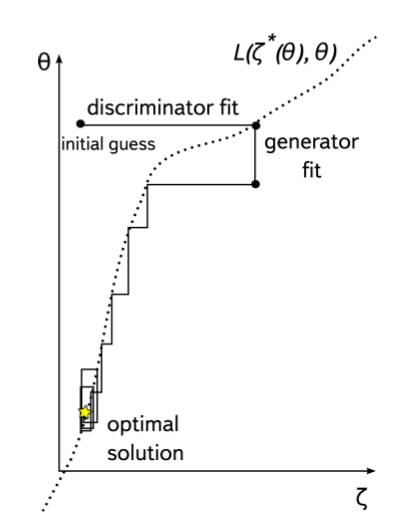
\includegraphics[width=0.4\linewidth]{5-GAN/gan-training}}
				\caption{Схематическое изображение процесса обучения GAN.}
				\label{5-gan-training}
			\end{figure}
	
		\subsubsection{Модификация ``pix2pix GAN''}
			Для решения задачи была опробована модификация обычной структуры GAN под названием ``pix2pix GAN'' \cite{pix2pix, p2p-vessnet}. Ее отличие от схемы GAN, введенной выше, состоит в том, что вместо шума на вход генератору приходят другие изображения, на которых он основывается при синтезе. Схематически ее устройство изображено на (Рис. \ref{5-p2p}).
	
			\begin{figure}[h!]
				\centering{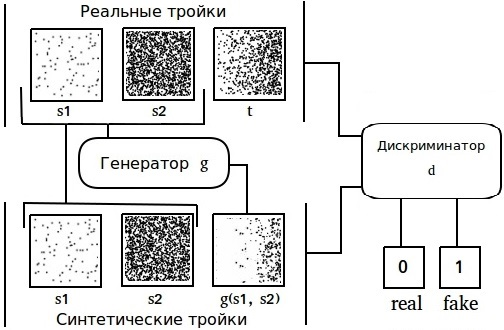
\includegraphics[width=0.75\linewidth]{5-GAN/p2p}}
				\caption{Схематическое устройство сети pix2pix GAN.}
				\label{5-p2p}
			\end{figure}
	
			Для pix2pix сети общий функционал потерь выглядит следующим образом: $$ L(G, D) = L_{adv}(G, D) + \eta L1$$
			$$L1 = \mathbb{E}_{p_{data}(s_1, s_2, r)} (\parallel r - G(s_1, s_2) \parallel_1)$$
			$$ L_{adv}(G, D) = \mathbb{E}_{p_{data}(s_1, s_2, r)}\log D(s_1, s_2, r) +  \mathbb{E}_{p_{data}(s_1, s_2)} \log (1 - D(s_1, s_2, G(s_1, s_2)))$$
			где G, D - генератор и дискриминатор, $(s_1, s_2, r)$ - тройка изображений (интенсивность слева, справа и реальное изображение с трендом),  $\mathbb{E}_{p_{data}(s_1, s_2, r)}$ - мат. ожидание логарифмического правдоподобия того, что тройка изображений $(s_1, s_2, r)$ принадлежит вероятностному распределению реальных троек $p_{data}(s_1, s_2, r)$, а $p_{data}(s_1, s_2)$ соответствует распределению реальных изображений $s_1, s_2$.
	
			В качестве генератора в \cite{pix2pix, p2p-vessnet} использовалась сеть ``U-Net'' \cite{unet}. Основное отличие сети ``U-Net'' от обычной сети архитектуры ``encoder-decoder'' заключается в наличии прямых связей между сверточными и разверточными слоями. Использование такого типа генератора позволяло увеличить качество синтезируемых изображений. Схемы сетей типа ``U-Net'' и ``Encoder-decoder'' приведены на (Рис. \ref{5-unet-sheme}).
			
			\begin{figure}[h!]
				\centering{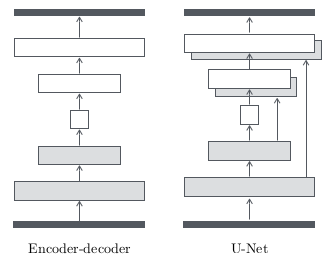
\includegraphics[width=0.5\linewidth]{5-GAN/unet-encoder}}
				\caption{Схематическое изображение нейросети-генератора.}
				\label{5-unet-sheme}.
			\end{figure}
			
			Разработанные и использованные в экспериментах архитектуры сетей генератора и дискриминатора были такими:\\
			Генератор:\\ C[nf]-C[nf*2]-C[nf*4]-C[nf*8]-C[nf*8]-C[nf*8]-C[nf*8]-C[nf*8]-DC[nf*8]-DC[nf*8]-DC[nf*8]-DC[nf*8]-DC[nf*4]-DC[nf*2]-DC[nf]-DC[1]\\
			Под С[nf] или DC[nf] здесь подразумеваются блоки, состоящие из сверточного или разверточного слоя с указанным числом фильтров, батч-нормализации и функции активации LeakyRELU с коэффициентом 0.2.\\
			Дискриминатор:\\
			C[nf]-C[nf*2]-C[nf*4]-C[nf*8]-C[1]\\
			В дискриминаторе батч-нормализация не применялась.
			
			При использовании ``U-Net'', к указанной выше архитектуре генератора добавлялись дополнительные сквозные связи между соответствующими сверточными и разверточными слоями.